\chapter{Problém maximálníhu řezu}

\section{Formulace úlohy}

Mějme neorientovaný graf $G = (V, E)$ s nezáporným ohodnocením hran $w$. Cílem je rozložit množinu vrcholů $V$ na nejvýše $k \geq 2$ disjunktních množin tak, aby součet hran vedoucí mezi různými množinamu byl maximální. Pokud $k = 2$ hovoříme o úloze \textbf{MAX CUT} a pro $k \geq 3$ o úloze \textbf{MAX $k$-CUT}.

\section{Úloha MAX CUT}

Nejprve se podíváme na aproximační algoritmus z článku \textbf{[REF]} pro úlohu MAX CUT.

\subsection*{Striktní kvadratický program pro MAX CUT}

\textbf{Kvadratický program} je problém optimalizace kvadratické funkce celočíselných proměnných, vzhledem ke kvadratickým omezením těchto proměnných. Je-li navíc každý monom (jednočlen) cenové funkce i daných omezení stupně $0$ nebo $2$, potom mluvíme o \textbf{striktním kvadratickém programu}.

Dále odvodíme striktní kvadratický program pro úlohu MAX CUT. Nechť $y_i \in \left\{ 1, -1 \right\}$ je proměnná příslušná vrcholu $i$. Množiny $S$ a $\bar{S}$ definujeme tak, že
$$
    S = \left\{ i \in V \mid y_i = 1 \right\}, \bar{S} = \left\{ i \in V \mid y_i = -1 \right\}.
$$
Pokud $i \in S$ a $j \in \bar{S}$, potom je součin $y_i y_j = -1$ a chceme, aby tato hrana přispívala hodnotou $w_{ij}$ k cenové funkci. Ve zbylých dvou možnostech je $y_i y_j = 1$ a chceme, aby se hodnota cenové funce nezměnila. Zakomponováním těchto podmínek definujeme striktní kvadratický program.

\begin{equation}\tag{SQ-MAX-CUT}
    \begin{split}
        OPT = &\max \frac{1}{2} \sum_{1 \leq i < j \leq n} w_{ij} (1 - y_i y_j) \\
        &\forall i \in V:\ y_i^2 = 1, \\
        &\forall i \in V:\ y_i \in \mathbb{Z}.
    \end{split}
    \label{eq:SQ-MAX-CUT}
\end{equation}


\subsection*{Vektorový program pro MAX CUT}

Poznamenejme jen, že úloha celočíselného programování je NP-těžká. Proto se dále budeme zabývat relaxací úlohy~\ref{eq:SQ-MAX-CUT}, což znamená, že upustíme od podmínek celočíselnosti a původní úlohu aproximujeme vektorovým programem. Modifikujeme tedy program~\ref{eq:SQ-MAX-CUT} tak, že každý součin $y_i y_j$ nahradíme skalárním součinem vektorů $\langle v_i, v_j \rangle$ v $\mathbb{R}^n$. Dostáváme následující vektorový program.

\begin{equation}\tag{V-MAX-CUT}
    \begin{split}
        RELAX = &\max \frac{1}{2} \sum_{1 \leq i < j \leq n} w_{ij} (1 - \langle v_i, v_j \rangle) \\
        &\forall i \in V:\ \langle v_i, v_i \rangle = 1, \\
        &\forall i \in V:\ v_i \in \mathbb{R}^n.
    \end{split}
    \label{eq:V-MAX-CUT}
\end{equation}


\subsection*{Semidefinitní program pro MAX CUT}

Vektorový program~\ref{eq:V-MAX-CUT} je ekvivalentní s příslušným semidefinitním programem. Nechť $W$ je vážená matice sousednosti grafu $G$ a $w_{ij}$ je váha hrany $ij$, kde $i < j$. Matice $J$ je matice $n \times n$ samých jedniček.

\begin{equation}\tag{SDP-MAX-CUT}
    \begin{split}
        RELAX = &\max \frac{1}{4} \langle W, J - Y \rangle \\
        &\forall i \in V:\ y_{ii} = 1, \\
        &Y \succeq 0.
    \end{split}
    \label{eq:SDP-MAX-CUT}
\end{equation}

\subsection*{Randomizovaný zaokrouhlovací algoritmus}

Mějme dva vektory $a_i, a_j$ optimálního řešení programu~\ref{eq:V-MAX-CUT}. Označme $\Theta_{ij}$ úhel, který tyto vektory svírají. Z podmínky
$$
    \forall i \in V:\ \langle v_i, v_i \rangle = 1
$$
dostáváme, že $\langle a_i, a_j \rangle = \cos \Theta_{ij}$ a příspěvěk těchto vektorů k optimálnímu řešení je
$$
    \frac{w_{ij}}{2} (1 - \cos \Theta_{ij}).
$$
Tedy čím \uv{blíž} je úhel $\Theta_{ij}$ hodnotě $\pi$, tím větší příspěvěk mají tyto vektory k hodnotě optimálního řešení. Dále si uvedeme algoritmus pro řešení úlohy MAX CUT a jeho analýzu.

\begin{alg}[MAX-CUT]$ $
    \begin{enumerate}
        \item Najdi řešení $a_1, \dots, a_n$ programu~\ref{eq:V-MAX-CUT}.
        \item Zvol náhodně vektor $r$ na jednotkové sféře $S_{n-1}$.
        \item $S = \left\{ i \in V \mid \langle a_i, r \rangle \geq 0 \right\}$.
    \end{enumerate}
    \label{alg:max-cut}
\end{alg}

Začneme dvěma lemmaty.

\begin{lm}
    Nechť $X_{ij}$ je jev takový, že vrcholy $i$ a $j$ jsou od sebe separovány, tj. jsou v různých množinách. Potom
    $$
        P\left[ X_{ij} \right] = \frac{\Theta_{ij}}{\pi}.
    $$
    \label{lemma:sep}
\end{lm}

\begin{proof}
    Vektory $a_i, a_j$ generují rovinu. Uvažme projekci náhodného vektoru $r$ na jednotkové sféře $S_{n-1}$ do této roviny. Potom vrcholy $i$ a $j$ jsou separovány, jestliže
    $$
        \langle a_i, a_j \rangle = \langle r, a_i \rangle + \langle r, a_j \rangle
    $$
    \begin{center}
        nebo
    \end{center}
    $$
        \langle a_i, a_j \rangle = \langle -r, a_i \rangle + \langle -r, a_j \rangle.
    $$
    Předchozí podmínku separace vrcholů ilustruje obrázek~\ref{fig:lemma_plane}.
\end{proof}

\begin{figure}[h!]
    \centering
    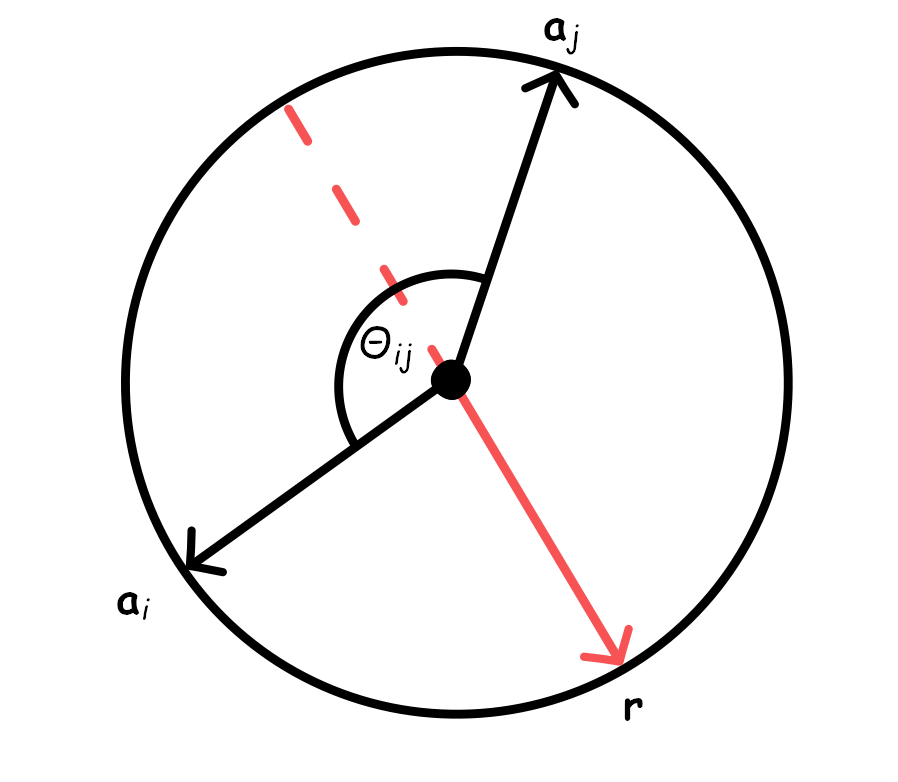
\includegraphics[width=0.5\textwidth]{img/lemma_plane.png}   
    \caption{Separace vrcholů $i$, $j$ náhodným vektorem $r$.}
    \label{fig:lemma_plane}
\end{figure}


\begin{lm}[KNUTH 2, 135]
    Nechť $x = (x_1, \dots, x_n)$ je vektor, jehož prvky jsou zvoleny nezávisle z normálního normovaného rozdělení $\mathcal{N}(0,1)$. Potom $r = \frac{x}{\| x \|}$ je náhodný vektor, který leží na jednotkové sféře $S_{n-1}$.
\end{lm}

Dále ukážeme, jak \uv{dobrou} aproximaci algoritmem~\ref{alg:max-cut} dostaneme. Označme
$$
    \alpha = \min_{0 \leq \Theta \leq \pi} \frac{2 \Theta}{\pi (1 - \cos \Theta)}.
$$
Snadno se ukáže, použitím derivace, že $\alpha \approx 0.87856$.

\begin{lm}
    Nechť $Y$ je náhodná veličina, která označuje součet vah hran, které vedou z $S$ do $\bar{S}$, nalezeny algoritmem~\ref{alg:max-cut}. Potom
    $$
        E\left[ Y \right] \geq \alpha \cdot RELAX.
    $$
\end{lm}

\begin{proof}
    Z definice čísla $\alpha$, pro $0 \leq \Theta \leq \pi$, dostáváme
    \begin{equation}
        \frac{\Theta}{\pi} = \frac{2 \Theta}{\pi (1 - \cos \Theta)} \cdot \frac{1 - \cos \Theta}{2} \geq \frac{\alpha}{2} (1 - \cos \Theta).
        \label{eq:proof_1}
    \end{equation}
    Použitím lemmatu~\ref{lemma:sep} a nerovnosti~\ref{eq:proof_1} dostáváme
    \begin{equation*}
        \begin{split}
            E\left[ Y \right] &= \sum w_{ij} P\left[ X_{ij} \right] \\
                              &= \sum w_{ij} \frac{\Theta_{ij}}{\pi} \\
                              &\geq \frac{\alpha}{2} \sum w_{ij} (1 - \cos \Theta_{ij}) \\
                              &= \alpha \cdot RELAX.
        \end{split}
    \end{equation*}
\end{proof}

\noindent Poznamenejme, že samozřejmě platí
\begin{equation}
    OPT \geq E\left[ Y \right] \geq \alpha \cdot RELAX.
    \label{eq:int-gap}
\end{equation}

\noindent Dále definujeme \textbf{mezeru celočíselnosti} relaxace (pro maximalizační problém) jako
$$
    \inf_{I} \frac{OPT(I)}{RELAX(I)},
$$
kde infimum probíhá přes všechny instance $I$ daného programu (pro minimalizační problém by se čitatel a jmenovat prohodily). Ze vztahu~\ref{eq:int-gap} dostáváme, že mezera celočíselnosti relaxace~\ref{eq:V-MAX-CUT} je alespoň $\alpha \approx 0.87856$.

Předchozí odvození je založeno na střední hodnotě náhodné veličiny $Y$. Proto kroky \textbf{2} a \textbf{3}, v algoritmu~\ref{alg:max-cut}, opakujeme vícekrát a jako výsledek zvolíme množinu $S$, která dává největší součet hran z $S$ do $\bar{S}$. Dále jen specifikujeme kolikrát musíme tyto kroky opakovat. Kompletní odvození je v \textbf{[REF]}. Zvolíme tedy $\varepsilon > 0$ (malé), nechť
$$
    c = \frac{\varepsilon \alpha}{2 + 2\varepsilon - \alpha},
$$
a kroky \textbf{2}, \textbf{3} opakujeme $\lceil \frac{1}{c} \rceil$-krát.


\section{Úloha MAX $k$-CUT}

V následující části si představíme semidefinitní (vektorové) formulace s aproximačními schématy z několika článků pro úlohu MAX~$k$-CUT a provedeme experiment, ve kterém je porovnáme na náhodném grafu.

\subsection{Frieze-Jerrum a MAX $k$-CUT \textbf{[REF]}}

\subsubsection*{Formulace}

Uvažujme rovnostranný simplex $\Sigma_k$ v $\mathbb{R}^{k-1}$ s vrcholy $b_1, b_2, \dots, b_k$. Nechť $c = (b_1 + \dots + b_k) / k$ je těžiště $\Sigma_k$ a nechť $a_i = b_i - c$, kde $i = 1, \dots, k$. Dále předpokládejme, že délka strany $\Sigma_k$ je taková, že $\| a_i\| = 1$.

\begin{lm}\textbf{[REF]}
    Pro $i \neq j$, platí
    $$
        \langle a_i, a_j \rangle = -\frac{1}{k-1}.
    $$
\end{lm}

\noindent Nyní můžeme formulovat úlohu MAX $k$-CUT následovně:

\begin{equation}\tag{FJ}
    \begin{split}
        &\max \frac{k-1}{k} \sum_{1 \leq i < j \leq n} w_{ij} (1 - \langle y_i, y_j \rangle) \\
        &y_i \in \left\{ a_1, \dots, a_k \right\}.
    \end{split}
    \label{eq:FJ}
\end{equation}

\noindent Poznamenejme, že
$$
    1 - \langle y_i, y_j \rangle = 
    \begin{cases}
        0           & y_i = y_j, \\
        k / (k - 1) & y_i \neq y_j.
    \end{cases}
$$

K získání vektorové relaxace programu~\ref{eq:FJ} nahradíme vektor $y_i$ vektorem $v_i$, kde $v_i$ je vektor na $S_{n-1}$.

\begin{equation}\tag{FJ-RELAX}
    \begin{split}
        &\max \frac{k}{k-1} \sum_{1 \leq i < j \leq n} w_{ij} (1 - \langle v_i, v_j \rangle) \\
        &\forall i \in V:\ \langle v_i, v_i \rangle = 1, \\
        &\forall i \neq j \in V:\ \langle v_i, v_j \rangle \geq -\frac{1}{k-1}, \\
        &\forall i \in V:\ v_i \in \mathbb{R}^n.
    \end{split}
    \label{eq:FJ-RELAX}
\end{equation}


\subsubsection*{Aproximační schéma}

Zvolíme $k$ náhodných vektorů $z_1, \dots, z_k$ na jednotkové sféře $S_{n-1}$. Pro každý vrchol $i \in V$ určíme $k$ skalárních součinů $\langle v_i, z_1 \rangle, \dots, \langle v_i, z_k \rangle$ a vrchol $i$ přidáme do množiny $V_j$, kde $j = \arg \max \left\{ \langle v_i, x_l \rangle \mid l = 1, \dots, k \right\}$.


\subsection{Goemans-Williamson a MAX $3$-CUT \textbf{[REF]}}

\subsubsection*{Formulace}

\begin{equation}\tag{GW-RELAX}
    \begin{split}
        &\max \frac{2}{3} \sum_{1 \leq i < j \leq n} w_{ij} (1 - \langle v_i^1, v_j^1 \rangle) \\
        &\forall i \in V\ \forall a,b \in \left\{ 1,2,3 \right\}, a \neq b:\ \langle v_i^a, v_i^b \rangle = -\frac{1}{2}, \\
        &\forall i,j \in V\ \forall a,b,c \in \left\{ 1,2,3 \right\}:\ \langle v_i^a, v_i^b \rangle = \langle v_i^{a+c}, v_i^{b+c} \rangle \\
        &\forall i,j \in V\ \forall a,b \in \left\{ 1,2,3 \right\}:\ \langle v_i^a, v_j^b \rangle \geq -\frac{1}{2} \\
        &\forall i \in V\ \forall a \in \left\{ 1,2,3 \right\}:\ \langle v_i^a, v_i^a \rangle = 1 \\
        &\forall i \in V\ \forall a \in \left\{ 1,2,3 \right\}:\ v_i^a \in \mathbb{R}^{3n}
    \end{split}
    \label{eq:GW-RELAX}
\end{equation}

\subsubsection*{Aproximační schéma}

Mějme $3n$ vektorů, které tvoří řešení \ref{eq:GW-RELAX}. Pro vrchol $i \in V$ leží vektory $v_i^1, v_i^2, v_i^3$ ve stejné rovině tak, že jsou otočeny o $\frac{2\pi}{3}$. Nejprve zvolíme vektor $g \in \mathbb{R}^{3n}$ takový, že každá složka je vybrána nezávisle z normálního normovaného rozdělení $\mathcal{N}(0,1)$. Pro každý vrchol $i \in V$ uděláme projekci vektoru $g$ do příslušné roviny. Odtud dostaneme úhel $\theta_i \in \langle 0, 2\pi)$ pro každý vrchol. Náhodně zvolíme úhel $\psi \in \langle 0, \pi)$ a vrchol $i \in V$ přidáme do množiny $V_j$, jestliže
$$
    \theta_i \in \psi + \frac{j 2 \pi}{3}, j \in \left\{ 0, 1, 2 \right\},
$$
kde úhly počítáme modulo $2$.

\subsection{de Klerk-Pasechnik-Warners a MAX $k$-CUT \textbf{[REF]}}

\subsubsection*{Formulace}

\begin{equation}\tag{THETA-$\bar{G}$}
    \begin{split}
        &\min t \\
        &\forall ij \in E:\ U_{ij} = -\frac{1}{t - 1} \\
        &\forall i \in V:\ U_{ii} = 1 \\
        &U \succeq 0, k \geq 2.
    \end{split}
    \label{eq:THETA-BAR-G}
\end{equation}

\subsubsection*{Aproximační schéma}

Mějme optimální řešení $(U, \vartheta(\bar{G}))$ programu \ref{eq:THETA-BAR-G}. Nechť
\begin{equation}
    Y = U \otimes \frac{k}{k - 1} \left( I_k - \frac{1}{k} e_k e_k^T \right).
\end{equation}

Uvažujeme rozklad matice $Y = V^T V$, kde $V = \left[ v_1^1\ v_1^2\ \dots\ v_1^k\ \dots\ v_n^k \right]$. Zvolíme náhodný jednotkový vektor $g \in \mathbb{R}^{kn}$ na sféře v $\mathbb{R}^{kn}$. Potom
$$
    x_i^p = 
    \begin{cases}
        1  & r^T v_i^p = \max \left\{ \langle g, v_i^q \rangle \mid q = 1, \dots, k \right\}, \\
        -1 & \text{jinak.}
    \end{cases}
$$


\subsection{Newman a MAX $k$-CUT \textbf{[REF]}}

\subsubsection*{Formulace}

Používá formulaci \ref{eq:FJ-RELAX}.

\subsubsection*{Aproximační schéma 1}

Následující aproximační schéma zobecňuje přístup z \textbf{[REF]}. Vyřešením programu~\ref{eq:FJ-RELAX} dostaneme řešení $v_1, \dots, v_n$. Pro každý vrchol $i \in V$ definujeme dva vektory v $\mathbb{R}^{2n}$
$$
    u_i = \left( v_i, 0 \right), u_i^\bot = \left( 0, v_i \right).
$$
$2$-dimenzionální disk je množina vektorů
$$
    u_i(\theta) = u_i \cos \theta + u_i^\bot \sin \theta, \theta \in \langle 0, \pi).
$$
Dále zvolíme náhodný vektor $g \in \mathbb{R}^{2n}$, kde každá složka je vybrána náhodně z normálního normovaného rozdělení $\mathcal{N}(0,1)$. Pro každý vrchol $i \in V$ uděláme projekci vektoru $g$ na disk $\left\{ u_i(\theta) \mid \theta \in \langle 0, \pi ) \right\}$ a určíme úhly
$$
    \theta_i = \arctan \left( \frac{\langle g, u_i^\bot \rangle}{\langle g, u_i \rangle} \right), \langle g, u_i \rangle \geq 0, \langle g, u_i^\bot \rangle \geq 0,
$$
$$
    \theta_i = \arctan \left( \frac{\langle g, u_i^\bot \rangle}{\langle g, u_i \rangle} \right) + \pi, \langle g, u_i \rangle \leq 0, \langle g, u_i^\bot \rangle \geq 0,
$$
$$
    \theta_i = \arctan \left( \frac{\langle g, u_i^\bot \rangle}{\langle g, u_i \rangle} \right) + \pi, \langle g, u_i \rangle \geq 0, \langle g, u_i^\bot \rangle \leq 0,
$$
$$
    \theta_i = \arctan \left( \frac{\langle g, u_i^\bot \rangle}{\langle g, u_i \rangle} \right) + 2\pi, \langle g, u_i \rangle \leq 0, \langle g, u_i^\bot \rangle \leq 0.
$$

Pro každý vrchol $i \in V$ máme tedy úhel $\theta_i$. Náhodně zvolíme úhel $\psi \in \langle 0, 2 \pi )$ a vrchol $i \in V$ přidáme do množiny $V_j$, jestliže
$$
    \theta_i \in \psi + \frac{j 2 \pi}{k}, j \in \left\{ 0, 1, \dots, k-1 \right\},
$$
kde úhly počítáme modulo $2$.


\subsubsection*{Aproximační schéma 2}

Princip je podobný, akorát pro každý vrchol $i \in V$ zvolíme $k-1$ náhodných vektorů $g_1, \dots, g_k$ takových, že každá složka každého vektoru je vybrána náhodně z normálního normovaného rozdělení $\mathcal{N}(0,1)$. Pro každý vrchol $i \in V$ určíme vektor
$$
    \left( \langle g_1, v_i \rangle, \dots, \langle g_{k-1}, v_i \rangle \right) \in \mathbb{R}^{k-1}.
$$
Každý z těchto vektorů je přiřazen nejbližšímu vrcholu $\Sigma_k$.

\subsection{Porovnání algoritmů}

Pro účely experimentu byl vygenerován náhodný graf $G=(V,E)$ se $100$ vrcholy, kde
$$
    \forall i,j \in V:\ P\left[ ij \in E \right] = 0.5.
$$

\subsubsection*{Aproximační poměry}
\begin{center}
    \begin{tabular}{ c c c c c }
    $k$  & FJ         & GW                  & dKPW                & N1         \\
    \hline
    $3$  & $0.832718$ & $\mathbf{0.836008}$ & $\mathbf{0.836008}$ &            \\  
    $4$  & $0.850304$ &                     & $\mathbf{0.857487}$ & $0.846478$ \\
    $5$  & $0.874243$ &                     & $\mathbf{0.876610}$ & $0.862440$ \\
    $10$ & $0.926642$ &                     & $\mathbf{0.926788}$ & $0.915885$ \\
    \end{tabular}
\end{center}

\subsubsection*{Experiment -- $10$ iterací}
\begin{center}
    \begin{tabular}{ c c c c c }
    $k$ & FJ         & GW                  & N1                  & N2         \\
    \hline
    $3$ & $1822$     & TODO                &                     &            \\  
    $4$ & $2006$     &                     & $1875$              & TODO       \\
    $5$ & $2121$     &                     & $2008$              & TODO       \\
    $6$ & $2172$     &                     & $2069$              & TODO       \\
    $7$ & $2222$     &                     & $2141$              & TODO       \\
    \end{tabular}
\end{center}

\subsubsection*{Experiment -- $100$ iterací}
\begin{center}
    \begin{tabular}{ c c c c c }
    $k$ & FJ         & GW                  & N1                  & N2         \\
    \hline
    $3$ & TODO       & TODO                &                     &            \\  
    $4$ & TODO       &                     & TODO                & TODO       \\
    $5$ & TODO       &                     & TODO                & TODO       \\
    $6$ & TODO       &                     & TODO                & TODO       \\
    $7$ & TODO       &                     & TODO                & TODO       \\
    \end{tabular}
\end{center}


\subsubsection*{Experiment -- $1000$ iterací}
\begin{center}
    \begin{tabular}{ c c c c c }
    $k$ & FJ         & GW                  & N1                  & N2         \\
    \hline
    $3$ & TODO       & TODO                &                     &            \\  
    $4$ & TODO       &                     & TODO                & TODO       \\
    $5$ & TODO       &                     & TODO                & TODO       \\
    $6$ & TODO       &                     & TODO                & TODO       \\
    $7$ & TODO       &                     & TODO                & TODO       \\
    \end{tabular}
\end{center}


\subsubsection*{Experiment -- $10000$ iterací}
\begin{center}
    \begin{tabular}{ c c c c c }
    $k$ & FJ         & GW                  & N1                  & N2          \\
    \hline
    $3$ & TODO       & TODO                &                     &            \\  
    $4$ & TODO       &                     & TODO                & TODO       \\
    $5$ & TODO       &                     & TODO                & TODO       \\
    $6$ & TODO       &                     & TODO                & TODO       \\
    $7$ & TODO       &                     & TODO                & TODO       \\
    \end{tabular}
\end{center}
